\documentclass[]{article}
\usepackage[UTF8]{ctex}
\usepackage{graphicx}
\usepackage{appendix}
\usepackage{geometry}
\usepackage{amsmath}
\usepackage{cite}
\usepackage{natbib}
\usepackage{listings}
\usepackage{titlesec}
\usepackage{float}
\usepackage{enumitem}
\usepackage[labelfont=bf]{caption}
\usepackage{listings}
\usepackage{hyperref}  
\usepackage[section]{placeins}
\usepackage{fix-cm}
\hypersetup{hidelinks,
	colorlinks=true,
	allcolors=black,
	pdfstartview=Fit,
	breaklinks=true
}

\lstset{
    basicstyle=\ttfamily,
    breaklines=true,
    frame=single,
    numbers=left,
    numberstyle=\tiny,
    language=[LaTeX]TeX
}

%opening

% Set ctex labels to English
\ctexset{
    contentsname = {Contents},
    figurename = {Figure},
    tablename = {Table},
    appendixname = {Appendix},
    abstractname = {Abstract},
    indexname = {Index},
    proofname = {Proof}
}

\begin{document}

\title{\huge Design of data encryption system}
\author{\large }
\date{}

\maketitle

\vspace{3cm}

\begin{center}
    {\large
        \begin{tabular}{|p{2.5cm}|p{3.5cm}|p{2.5cm}|p{3.5cm}|}
            \hline
            \textbf{Name}     &  & \textbf{Class} &       \\[0.8cm]
            \hline
            \textbf{Date}     &  & \textbf{Score} & \quad \\[0.8cm]
            \hline
            \textbf{Examiner} &  & \quad          & \quad \\[0.8cm]
            \hline
        \end{tabular}
    }
\end{center}

\newpage
\tableofcontents
\newpage

\section{Introduction}
The full adder is a fundamental digital logic circuit used in arithmetic operations. It is capable of adding three binary digits and produces a sum and a carry-out. This experiment focuses on the design, implementation, and simulation of full adders using VHDL on an FPGA platform using Quartus II and ModelSim simulation tools.

\section{Experiment Procedure}

\subsection{Project Setup and Environment Configuration}
\begin{enumerate}[label = (\arabic*)]
    \item Launch Quartus II 13.0 software to begin the FPGA design project.
    \item Create a new project through the "New Project Wizard" interface. Configure the project as follows:
          \begin{itemize}
              \item Project name: \textit{fadd4}
              \item Configure the top-level entity as the testbench module
          \end{itemize}
    \item For simulation-only applications, allow Quartus II to auto-select the default FPGA device.
    \item Set up the ModelSim simulation environment with appropriate libraries and simulation settings.
\end{enumerate}

\subsection{Full Adder Design and Implementation}
\noindent A full adder is a digital circuit that performs the addition of three binary bits: two operands (A and B) and a carry-in (Cin). It produces two outputs: a sum (S) and a carry-out (Cout).

\subsubsection{Full Adder Logic}
The truth table for a full adder is:
\begin{center}
    {\small
        \begin{tabular}{|c|c|c|c|c|}
            \hline
            A & B & Cin & S & Cout \\
            \hline
            0 & 0 & 0   & 0 & 0    \\
            0 & 0 & 1   & 1 & 0    \\
            0 & 1 & 0   & 1 & 0    \\
            0 & 1 & 1   & 0 & 1    \\
            1 & 0 & 0   & 1 & 0    \\
            1 & 0 & 1   & 0 & 1    \\
            1 & 1 & 0   & 0 & 1    \\
            1 & 1 & 1   & 1 & 1    \\
            \hline
        \end{tabular}
    }
\end{center}

\subsubsection{VHDL Implementation}
\noindent The following VHDL code implements a single full adder cell:

\begin{lstlisting}[language = VHDL]
LIBRARY IEEE; 
USE IEEE.std_logic_1164.ALL; 
ENTITY fadd IS 
    PORT (a,b,ci: IN std_logic; 
    co,sum: OUT std_logic 
    ); 
END fadd; 

ARCHITECTURE dataflow OF fadd IS 
BEGIN 
co<=(a and b)or(b and ci)or(a and ci); 
sum<=a xor b xor ci; 
END dataflow; 
\end{lstlisting}

\begin{figure}[H]
    \centering
    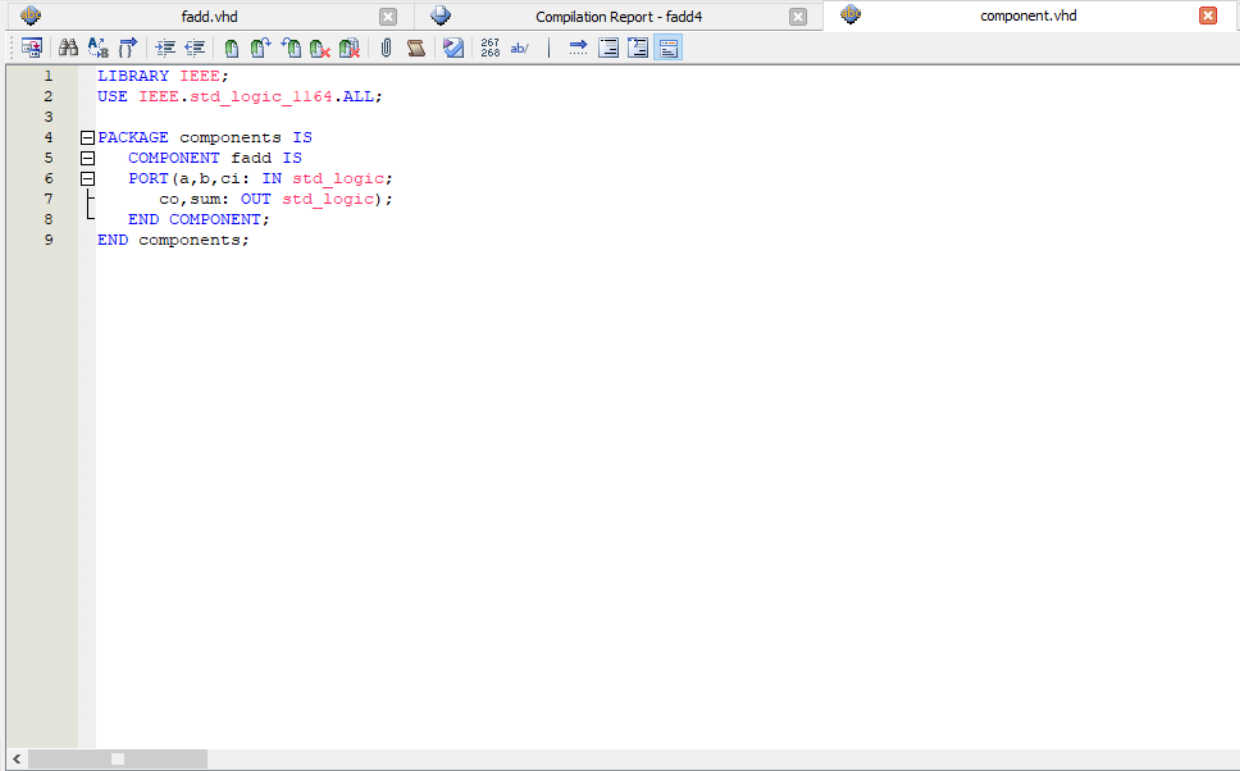
\includegraphics[width=1.0\linewidth]{component.jpg}
    \caption{single full adder}
    \label{fig:component}
\end{figure}

\subsection{4-Bit Full Adder Design}
\noindent For multi-bit addition operations, we extend the single full adder to create a 4-bit full adder by cascading four individual full adder cells:

\begin{lstlisting}[language = VHDL]
LIBRARY IEEE;
USE IEEE.std_logic_1164.ALL;
USE work.components.ALL;

ENTITY fadd4 IS
    PORT (
        a   : IN  std_logic_vector(3 DOWNTO 0);
        b   : IN  std_logic_vector(3 DOWNTO 0);
        ci  : IN  std_logic;
        co  : OUT std_logic;
        sum : OUT std_logic_vector(3 DOWNTO 0)
    );
END fadd4;

ARCHITECTURE stru OF fadd4 IS
    SIGNAL ci_ns : std_logic_vector(2 DOWNTO 0);
BEGIN
    fa0: fadd
        PORT MAP (
            a   => a(0),
            b   => b(0),
            ci  => ci,
            co  => ci_ns(0),
            sum => sum(0)
        );

    fa1: fadd
        PORT MAP (
            a   => a(1),
            b   => b(1),
            ci  => ci_ns(0),
            co  => ci_ns(1),
            sum => sum(1)
        );

    fa2: fadd
        PORT MAP (
            a   => a(2),
            b   => b(2),
            ci  => ci_ns(1),
            co  => ci_ns(2),
            sum => sum(2)
        );

    fa3: fadd
        PORT MAP (
            a   => a(3),
            b   => b(3),
            ci  => ci_ns(2),
            co  => co,
            sum => sum(3)
        );
END stru;
\end{lstlisting}

\begin{figure}[H]
    \centering
    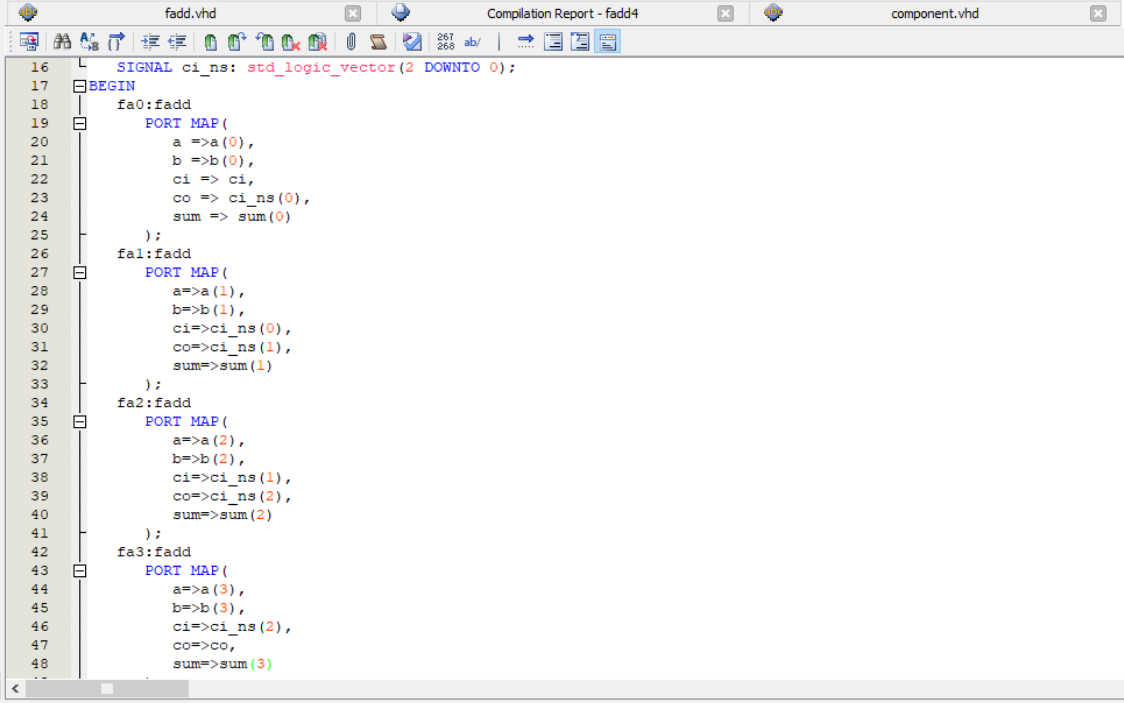
\includegraphics[width=1.0\linewidth]{fadd4.jpg}
    \caption{4-bit full adder}
    \label{fig:fadd4}
\end{figure}

\subsection{Testbench Development}
\noindent At this time, we need to modify it based on the previously generated testbench template, that is, we need to add the following code to the vht file：

\begin{lstlisting}[language = VHDL]
BEGIN
    -- code that executes only once
    a<="0000";
    b<="0000";
    ci<='0';
    for k in 0 to 1 loop
        for j in 0 to 3 loop
            for i in 0 to 3 loop
                wait for 10 ns;
                a<=a+1;
            end loop;
            b<=b+1;
        end loop;
        ci<=not ci;
    end loop;
WAIT;
END PROCESS init;
always : PROCESS
\end{lstlisting}

\begin{figure}[H]
    \centering
    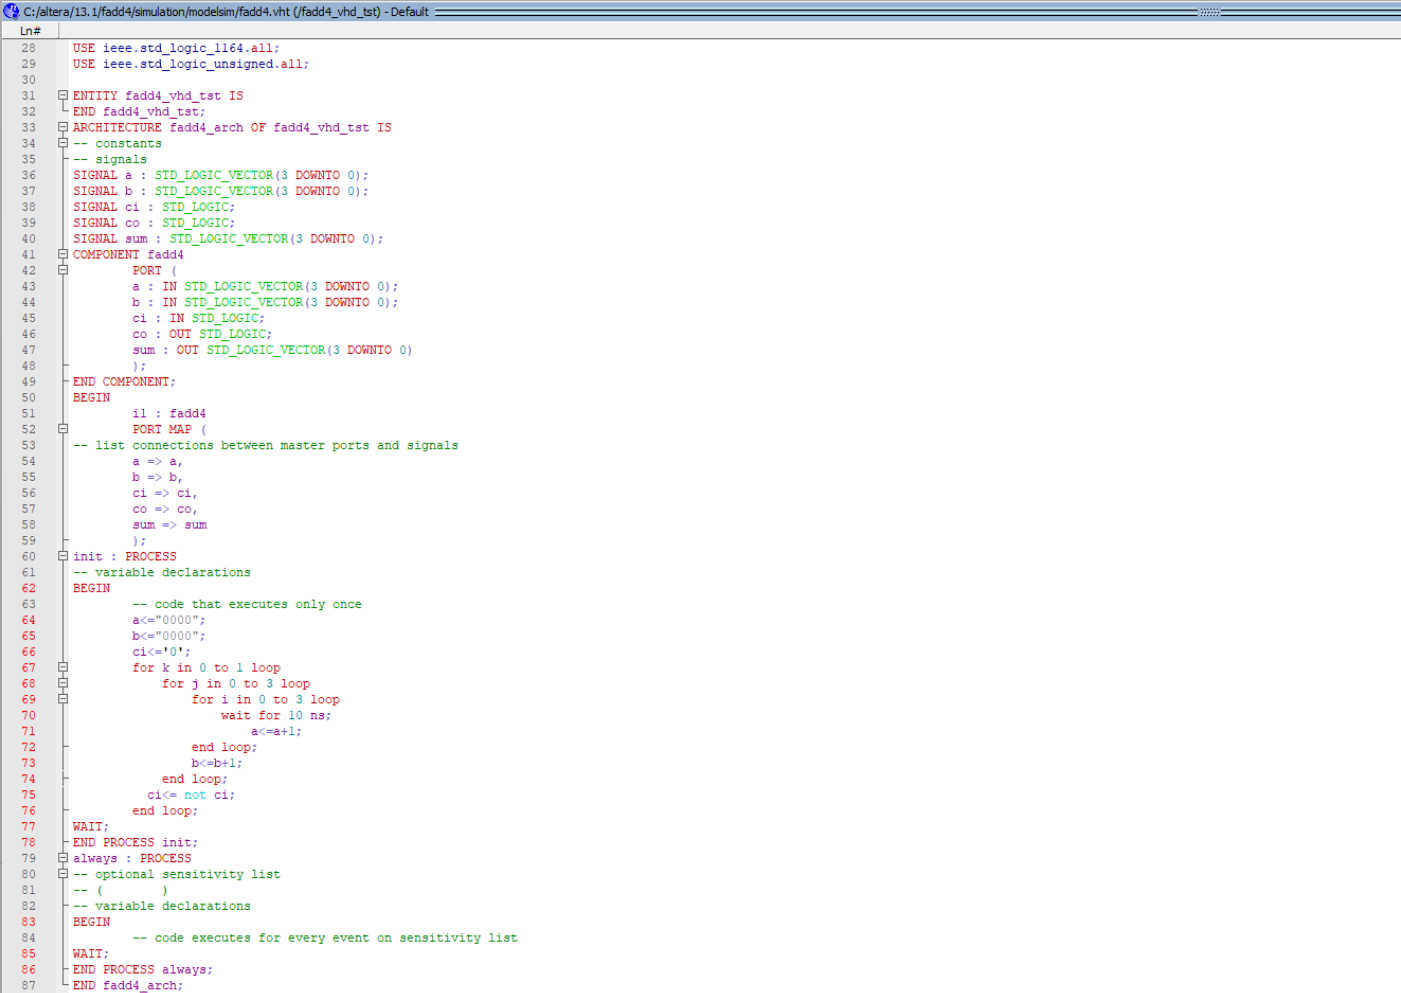
\includegraphics[width=1.0\linewidth]{fadd4_vht.jpg}
    \caption{testbench for 4-bit full adder}
    \label{fig:fadd4_vht}
\end{figure}

\subsection{Design Compilation and Synthesis}
\begin{enumerate}[label = (\arabic*)]
    \item Compile all VHDL source files to check for syntax errors and generate compiled design files.
    \item Analyze the post-synthesis reports to verify correct logic implementation.
    \item Generate Resource Usage Reports to optimize area and timing performance.
    \item Create netlist files for simulation and FPGA implementation.
\end{enumerate}
\section{Experimental Results and Analysis}

\subsection{Simulation Waveforms}
\noindent The following waveforms demonstrate the functional behavior of the 4-bit full adder during simulation:

\begin{figure}[H]
    \centering
    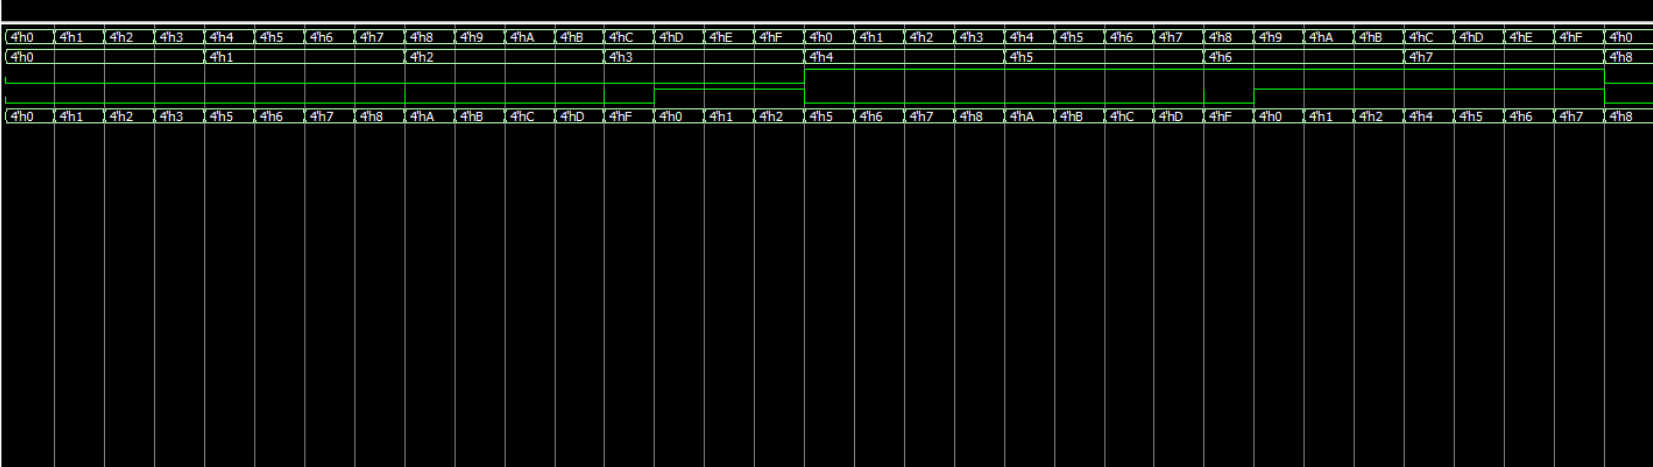
\includegraphics[width=1.0\linewidth]{wave1.jpg}
    \caption{Simulation Waveforms 1}
    \label{fig:wave1}
\end{figure}

\begin{figure}[H]
    \centering
    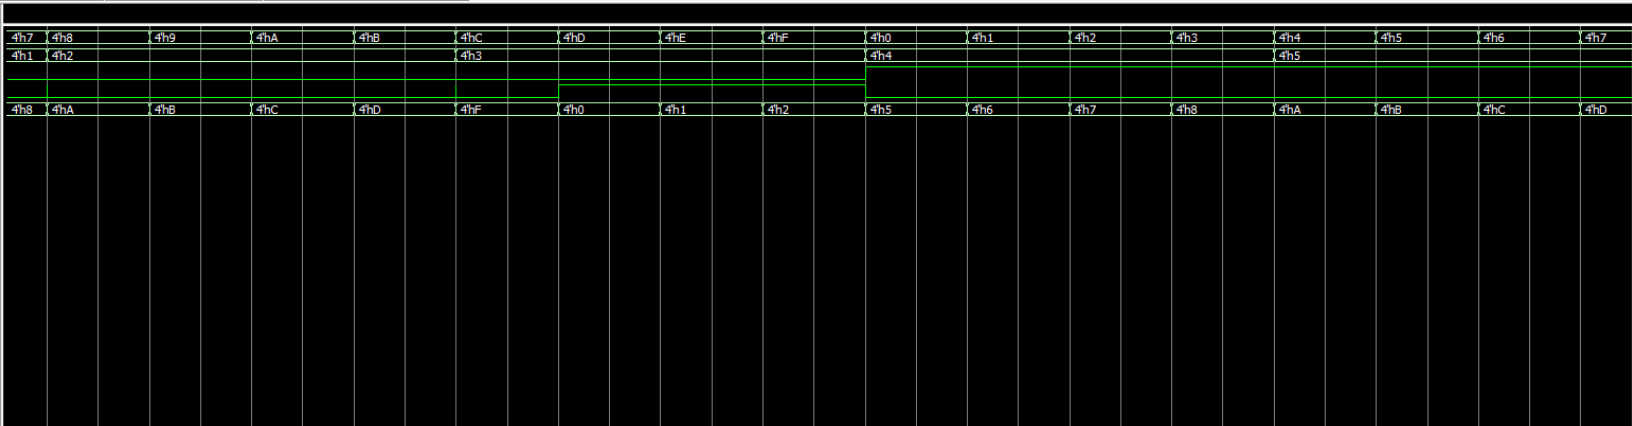
\includegraphics[width=1.0\linewidth]{wave2.jpg}
    \caption{Simulation Waveforms 2(same as wave1 but zoomed in)}
    \label{fig:wave2}
\end{figure}

\subsection{Conclusion}
\begin{enumerate}
    \item The simulation waveform successfully verifies the correctness of the 4-bit full adder, with the output values for both the sum and carry matching the expected results precisely. However, the simulation waveform displays some glitches. These glitches are likely due to the fact that "Enable Optimization" was not selected during the simulation. Without optimization, the simulation assumes an idealized model of the circuit, where all components react instantaneously. In reality, however, each unit or logic gate in the circuit has a propagation delay, meaning that the signal changes at slightly different times depending on the gate’s internal characteristics.

    \item This delay, which varies across different logic elements in the design, can cause temporary inconsistencies or glitches in the output waveform. These glitches are artifacts of the simulation environment, which does not fully account for the real-world behavior of the circuit, such as signal timing and the delays inherent in physical components. Enabling the optimization feature would make the simulation more reflective of the actual circuit behavior, reducing these glitches by better modeling the propagation delay and the timing characteristics of the logic gates involved.

\end{enumerate}

\end{document}